\chapter{Marco teórico} \label{section-marco-teorico}
\markright{Marco teórico}

\paragraph{} A continuación, se presentarán los conceptos fundamentales que apoyan al desarrollo y análisis experimental llevado a cabo en este proyecto de grado, involucrando principalmente conceptos de aprendizaje automático.

\section{Aprendizaje automático}

\paragraph{}Aprendizaje automático es un campo de las ciencias de la computación y una rama de la inteligencia artificial dedicada a desarrollar técnicas que permitan construir programas que mejoran de forma automática basados en la experiencia, se dice que estos programas \textit{aprenden} con la experiencia. En términos formales, el concepto de que un programa \textit{aprenda} es puesto en palabras por \citet{mitchell1997machine} de la siguiente mantera: \textit{“Se dice que un programa de computadora aprende de la experiencia E con respecto a una tarea T y medida de desempeño P si su desempeño en la tarea T, medida en términos de P, mejora con la experiencia E”}. 

\paragraph{}Los algoritmos de aprendizaje automático pueden ser clasificados en algoritmos de aprendizaje supervisado y no supervisado en función de la necesidad de la existencia de datos previos que oficien de experiencias. En aprendizaje supervisado las entradas del algoritmo son ejemplos de experiencias (conocidos como datos de entrenamiento) y sus respectivas salidas, de tal manera, el algoritmo aprende reglas generales de mapeo entre entradas y salidas. Ejemplos de algoritmos de aprendizaje supervisado son las \textit{redes neuronales con propagación hacia atrás} , así como las \textit{máquinas de soporte vectorial} o los \textit{árboles de decisión}, entre otros. En algoritmos no supervisados no se ofrecen las salidas de los datos de entrenamiento, dejando a los algoritmos detectar patrones en los datos por sí mismo, el algoritmo \textit{K-Means} es un ejemplo de este tipo de aprendizaje automático. 

\paragraph{}También podemos encontrar algoritmos de aprendizaje por refuerzos. Dentro del aprendizaje automático, el aprendizaje por refuerzos se ocupa de estudiar cómo agentes de software toman acciones en su entorno en función de maximizar una recompensa. Un ejemplo de este tipo de algoritmos es \textit{Q-Learning}, que implica el aprendizaje de una política que le indique al agente qué decisión tomar bajo cuáles circunstancias.

\paragraph{}Los problemas estudiados en aprendizaje automático pueden ser de clasificación o de regresión. Un problema se considera de clasificación cuando se puede clasificar a las instancias del problema de acuerdo a valores de un dominio discreto, como en el ejemplo de reconocimiento de flores mediante imágenes. Un problema se considera de regresión cuando se puede clasificar a las instancias del problema de acuerdo a valores de un dominio continuo, por ejemplo al intentar predecir el valor de una propiedad dado un conjunto de características asociadas a la misma.

\paragraph{}Las técnicas basadas en aprendizaje automático han tomando mayor relevancia en los últimos años debido al crecimiento de los volumenes y variedades de datos, disminución de los costos de infraestructura, acompañado por un crecimiento en capacidad computacional del hardware y capacidad de almacenamiento a precios accesibles. 

\paragraph{}En este proyecto trabajaremos con dos algoritmos de aprendizaje automático conocidos como \textit{máquina de soporte vectorial} y \textit{redes neuronales}, en un problema de clasificación.

\section{Clasificadores de interés}

\paragraph{}En el marco del aprendizaje automático supervisado, existen dos tipos de clasificadores de interés para este proyecto de grado. Estos son las redes neuronales y las máquinas de soporte vectorial (o SVM).

\subsection{Redes neuronales artificiales}

\paragraph{}Una red neuronal artificial es un algoritmo de aprendizaje automático utilizado tanto para problemas de clasificación como de regresión.
Su concepción está inspirada en la observación de los mecanismos de aprendizaje en sistemas biológicos.
Las redes neuronales artificiales están formadas por unidades más simples e interconectadas. 
Cada unidad tiene entradas reales y calcula una única salida (también real) mediante la asignación de pesos en regresiones lineales.
Estas unidades se denominan perceptrones.
Un perceptrón recibe valores de $n$ entradas $x_1, x_2, \dots x_n$, realiza una combinación lineal con ellos, obteniendo una expresión $x_1 w_1 + x_2 w_2 + \dots x_n w_n$ donde $w_i$ es el peso otorgado a $x_i$, para todo $i \in \{1, \dots, n\}$.
Esta expresión es evaluada con una función conocida como \textit{función de activación}, que devuelve un valor de acuerdo a si la combinación lineal de los valores de entrada supera un umbral determinado o no.
Por ejemplo, utilizando la función signo como función de activación, si la combinación lineal de los valores de entrada es mayor que cero, se devolverá $1$ como salida y $-1$ en caso contrario.
La Figura \ref{fig:perceptron} muestra la estructura de un perceptrón con función de activación signo.

\textsc{\begin{figure}[ht!]
	\centering
    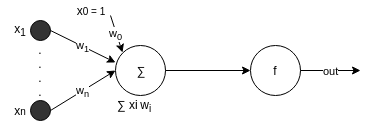
\includegraphics[width=.5\linewidth]{imagenes/perceptron.png}
	\caption{Perceptron con función de activación \textit{f = signo(x)}}
	\label{fig:perceptron}
\end{figure}}

\paragraph{}Cuando se calcula la combinación lineal de los valores de entrada, el valor resultante puede oscilar entre $-\infty$ y $+\infty$, dado que un perceptrón no posee una referencia de cuáles son los límites asociados a las posibles clases de clasificación para el problema de interés.
Las funciones de activación se utilizan con el propósito de limitar este valor al producir la salida del perceptrón. 

\paragraph{}El perceptrón puede ser utilizado para modelar funciones lógicas, como AND, OR, NAND y NOR, ajustando la cantidad de entradas según la cantidad de entradas de la función lógica y ajustando los pesos de tal manera que las salidas sean $1$ y $-1$.
La capacidad de los perceptrones para representar funciones lógicas es relevante puesto que da lugar a que cualquier función lógica pueda ser representada mediante una red de perceptrones de dos niveles de profundidad, en la cual las entradas son conectadas a múltiples perceptrones y las salidas de estos son conectadas a la siguiente capa.
De todas maneras, múltiples capas de perceptrones, dada su naturaleza de unidades lineales, producirán funciones lineales.
Para expresar decisiones no lineales es necesario emplear neuronas cuyas salidas sean funciones no lineales de sus entradas.
Una posibilidad es la utilización de unidades sigmoide, cuya estructura es similar a la del perceptrón, variando en la función de activación, que es la función \textit{sigmoide}, una función no lineal diferenciable.
La personalización de las neuronas artificiales, por lo tanto, genera la posibilidad de representar una gran variedad de funciones.

\paragraph{}Por lo tanto, la forma de trabajar utilizando redes neuronales puede dividirse en dos fases.
Primero, se debe encontrar una configuración arquitectónica de perceptrones o neuronas capaz de expresar la función que se está intentando aprender (que puede no ser conocida a priori y, por lo tanto, puede ser necesario evaluar diversas disposiciones en términos de cantidad de capas y cantidad de neuronas).
Luego, se debe encontrar un vector de pesos $(w_0,w_1,\dots,w_n)$ apropiado para cada perceptrón mediante el entrenamiento. 
En el contexto de un problema de clasificación, entrenar una red neuronal consiste en administrarle ejemplos ya clasificados del problema de interés.
Para cada ejemplo administrado, la red primero producirá una clasificación para el problema dado y la comparará con la salida esperada, tras lo cual ajustará los pesos de cada una de sus unidades para reducir la eventual diferencia entre estos dos valores, utilizando un algoritmo definido previamente.
En este trabajo, donde se utilizan redes multicapa, se utiliza el algoritmo \textit{Backpropagation} para \textit{aprender} los vectores de pesos de cada una de las unidades interconectadas que las componen. 

% TODO hacer notar a renzo inconsistencia en correcciones
\paragraph{}Para describir el funcionamiento del algoritmo Backpropagation, y cómo este ajusta de manera iterativa los pesos de las unidades, es importante definir el concepto de \textit{gradiente descendente}.
Gradiente descendente es una técnica que busca encontrar un mínimo de una función, ya sea local o no. 
Para encontrar un mínimo local de una función usando gradiente descendente, se calcula el gradiente de la misma en un punto de partida y se lo hace variar en dirección negativa a dicho gradiente.
De esta manera, se llegará a un mínimo local eventualmente.
En el contexto de las redes neuronales, la búsqueda por gradiente descendente encuentra un vector de pesos que minimiza el error con respecto al hiperplano generado por los vectores de pesos asociados al conjunto de entrenamiento.
La búsqueda comienza utilizando un vector de pesos inicial arbitrario, modificándolo en pequeños pasos, realizando cada modificación de tal manera que se produzca una disminución en el error con respecto al hiperplano de pesos asociados a la solución.
Este proceso continúa hasta que se llega a un error global mínimo.
Gradiente descendente es una estrategia de búsqueda en un espacio grande o infinito de hipótesis que se puede aplicar siempre que dicho espacio contenga hipótesis que puedan ser determinadas de forma paramétrica, como son los pesos en las unidades.
Así también, se requiere que el error pueda ser diferenciado con respecto a estos parámetros.
Esta estrategia tiene algunas dificultades fundamentales; una de ellas es que la velocidad de convergencia a un mínimo es lenta, pudiendo requerir varios miles de pasos para lograrla y además, si existen varios mínimos locales en la superficie de error, no garantiza que la búsqueda converja a un mínimo global.

\paragraph{}El algoritmo Backpropagation es un método utilizado en redes multicapa para calcular el gradiente que se utiliza para el cálculo de los pesos de las neuronas, empleando gradiente descendente.
El error es calculado en la salida de la red multicapa y es distribuido \textit{hacia atrás}, hacia las capas internas de la red, calculando para cada unidad perteneciente a una capa intermedia su error y actualizando sus pesos.
El bucle de actualización de pesos en Backpropagation puede iterar miles de veces en una aplicación típica de redes neuronales, por lo que existen una variedad de criterios de terminación, como detener el bucle luego de una cantidad fija de iteraciones, o detener el bucle luego de que el error alcanza cierto umbral definido, o por criterios definidos sobre un conjunto dado de prueba. 
Los criterios de terminación son importantes y su elección es delicada dado que, de terminar antes de lo necesario con las iteraciones, la red neuronal puede devolver salidas con un error elevado.
Por otra parte, si se realizan muchas iteraciones se puede generar un sobreajuste de la red neuronal al conjunto de entrenamiento, produciendo resultados de bajo error para el conjunto de entrenamiento, pero con más altos niveles de error para conjuntos de validación con datos no vistos durante el entrenamiento.
Backpropagation no asegura la convergencia a un mínimo global debido al uso gradiente descendente en espacios de hipótesis de alta dimensionalidad (pudiendo haber tantas dimensiones como pesos).
La alta dimensionalidad incrementa la probabilidad de que los movimientos en la superficie de error no permitan alcanzar un mínimo global, pudiendo alcanzar mínimos para una o más dimensiones, que no sean necesariamente mínimos para las otras dimensiones.
A pesar de la falta de garantías con respecto a la convergencia del algoritmo a un mínimo global, Backpropagation es un método de aproximación de funciones altamente efectivo.
Una característica que manifiestan las redes neuronales entrenadas con Backpropagation es la habilidad de descubrir relaciones no triviales presentes en los datos de entrada, a nivel de las capas intermedias ocultas de la red.
Por ejemplo, dada una instancia de entrenamiento con $N$ atributos, la utilización de Backpropagation puede conducir a que se descubran relaciones entre los atributos $a_i$ y $a_j$,  $\forall i, j \in \{1, \dots, N\}, i \neq j$ no identificables por un humano a simple vista, y que contribuyen a la clasificación en gran medida.

\paragraph{}En este trabajo se construyen varios tipos de redes que varían en las funciones de activación utilizadas por las unidades.
A continuación se presentan las funciones de activación que se usaron durante este trabajo. 
La función \textit{tanh}, expresada de la siguiente manera: $f(x) = tanh(x) = \frac{2}{1 + e^{-2x}} - 1 $, es una función continua no lineal.
Al componerla consigo misma se obtienen funciones no lineales, lo que permite combinar a unidades con esta función de activación sin perder la no linealidad. 
tanh es una función suave en su curva, mostrando que pequeñas variaciones en valores del dominio cercanos a 0 generan cambios grandes en los valores correspondientes del codominio.
Esto implica que se le da una gran ponderación a los valores de los extremos del codominio, algo análogo a una tasa de aprendizaje. 

La función \textit{relu}, expresada de la siguiente manera: $f(x) = relu(x) = max(0, x)$ es no lineal y las composiciones de ella consigo misma son no lineales, pero por su forma, puede ocasionar que algunas neuronas den como resultado cero, constituyéndose una eventual pérdida de información.
Este problema se llama \textit{dying relu problem}.
Sin embargo, computar relu es menos costoso que computar tanh porque implica operaciones matemáticas más simples.
Por último, la función \textit{identity}, también llamada de activación lineal, expresada de la siguiente manera: $f(x) = identity(x) = x$, siempre retorna el mismo valor que recibe en su argumento, lo que implica que equivale a una regresión lineal utilizando los pesos de la unidad.

% Ventajas y desventajas
\paragraph{}Entre las ventajas de utilizar redes neuronales se encuentra el hecho de que se adecuan correctamente a problemas en los cuales los datos de entrenamiento contienen ruido y a contextos en los cuales tiempos largos de entrenamiento son aceptables.
Además, las redes neuronales suelen mantener tiempos bajos de clasificación.
Adicionalmente, como se menciona en la Sección \ref{section-trabajos-tecnicas-clasificacion}, una desventaja de las redes neuronales es que su representación interna es difícil de entender para los humanos y, por este motivo, se dice que se comportan como una “caja negra”.

\subsection{SVM}

\paragraph{}Una SVM o máquina de soporte vectorial es un algoritmo o clasificador de aprendizaje automático supervisado utilizado fundamentalmente para problemas de clasificación.
Dado un problema de aprendizaje automático supervisado de clasificación donde las instancias del problema pueden ser clasificadas en $N$ clases y un conjunto de ejemplos de entrenamiento de dicho problema, una SVM busca encontrar un hiperplano que los divida de manera lineal esas $N$ clases. De esta manera, frente a una nueva instancia del problema, la SVM será capaz de clasificarla generando una correspondencia entre esta instancia y una de las $N$ clases posibles.

\paragraph{}Se denominan vectores de soporte a aquellos ejemplos de entrenamiento más cercanos al hiperplano, la distancia entre el hiperplano y un vector de soporte se conoce como margen y para un conjunto de ejemplos de entrenamiento, SVM busca dividirlos de manera óptima con un hiperplano donde se maximice estos márgenes para cada uno de los vectores de soporte, cada uno asociado a su vez a una de las posibles clases de clasificación del problema. En un problema donde las instancias pueden ser clasificadas en dos clases, el hiperplano de dos dimensiones es representado por una línea recta y los vectores de soporte son aquellos ejemplos de entrenamiento más cercanos a ella, desde las dos direcciones posibles. La figura \ref{fig:svm_margin} muestra lo antedicho.

\textsc{\begin{figure}[ht!]
	\centering
    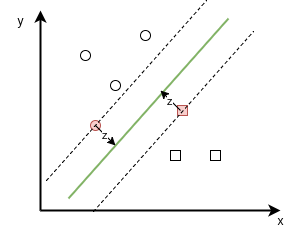
\includegraphics[width=.5\linewidth]{imagenes/svm_margenes.png}
	\caption{En esta figura se observan dos conjuntos de elementos (cuadrados y círculos), clasificados en dos clases, en base a dos características, \textit{x} e \textit{y}. El hiperplano generado por svm se muestra como la recta negra y se marcan los márgenes en lineas punteadas. Así, en color rojo se muestran los vectores de soporte, uno perteneciente a cada clase, siendo z la distancia entre cada vector de soporte y el hiperplano.}
	\label{fig:svm_margin}
\end{figure}}


\paragraph{}El hiperplano estará dado por la ecuación $g(\vec{x}) = \vec{w}^T\vec{x} + w_0$ donde $\vec{w}$ es un vector de pesos y $\vec{x}$ es el vector de características. La distancia a uno de los márgenes está dada por $z = \abs{g(\vec{x})} / \norm{\vec{w}} = 1 / \norm{\vec{w}}$, por lo que el margen total se computa como $1 / \norm{\vec{w}} +  1 / \norm{\vec{w}} = 2 / \norm{\vec{w}}$. Por lo tanto, minimizando la expresión $\norm{\vec{w}}$ se maximizan los márgenes, maximizando la separabilidad de las clases. La confianza en la clasificación de una instancia del problema estará dada por la distancia de dicha instancia al hiperplano de manera directamente proporcional.

\paragraph{}Cuando se tienen más de dos clases objetivo para la clasificación, se utiliza un SVM multiclase en el cual la técnica de aprendizaje admite dos posibles estrategias. Por un lado \textit{One vs. Rest} (\textit{OVR}) y por otro \textit{One vs. One} (\textit{OVO}). Dado un conjunto de $N$ clases $\{c_1,c_2,\dots,c_N\}$, \textit{OVR} intentará clasificar $c_i$ contra $\{c_1,c_2,\dots,c_{i-1},c_{i+1},\dots,c_{N - 1}\}$ dejando como representantes de la clase $C_N$ los datos que no fueron clasificado en las otras clases. Por otro lado \textit{OVO}, intentará clasificar cada clase $i$ contra cada $C_j \forall j \neq i$, creando un hiperplano para cada una de las combinaciones. Comparando las dos estrategias, \textit{OVR} genera $C_{N-1}$ clasificadores, en contraste con \textit{OVO} que generará una combinación de $N$ tomada de a dos, generando un número mayor de clasificadores que \textit{OVR}. Por otro lado, \textit{OVR} es más sensible al no balance de los datos, en el sentido de que si intento clasificar  y la cantidad de datos representantes de esta clase es baja en comparación con el total de datos, esta clase podría verse eclipsada por las demás. En cambio, con \textit{OVO} este fenómeno no se manifiesta en igual medida, dado que se generan clasificadores uno a uno. La figura \ref{fig:ovoovr} muestra lo antedicho.

\textsc{\begin{figure}[ht!]
	\centering
    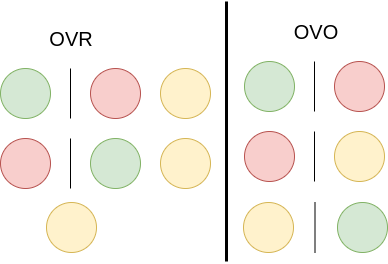
\includegraphics[width=.5\linewidth]{imagenes/ovoovr.png}
	\caption{A la izquierda se muestra la estrategia de entrenamiento de SVM \textit{OVR}, en la cual cada una de las clases se intenta clasificar contra el resto de las clases. A la derecha se muestra la estrategia \textit{OVO}, que genera clasificadores para cada par de clases.}
	\label{fig:ovoovr}
\end{figure}}

\paragraph{}La obtención de un hiperplano que divida de manera lineal a los ejemplos de entrenamiento no siempre es posible. Cuando no es posible, se suele utilizar una técnica conocida como \textit{kernelización} o \textit{Kernel Trick} para aumentar la dimensión del dominio donde se está buscando un hiperplano e intentar obtener un hiperplano que separe linealmente a los ejemplos de entrenamiento en esa dimensión. De esta manera, es posible clasificar a nuevas instancias del problema de acuerdo a este nuevo hiperplano y transformar la clasificación obtenida a la dimensión original del problema dada por las clases de clasificación disponibles. De todas maneras, una utilización imprudente del \textit{Kernel Trick} puede llevar a un sobreajuste del modelo.

\paragraph{}Entre las desventajas de utilizar SVM encontramos que los tiempos de entrenamiento asociados pueden ser significativos para grandes conjuntos de entrenamiento, pudiendo tener consumos considerables de memoria tanto en entrenamiento como en pruebas. Así también la selección de parámetros de \textit{Kernel} para el realizar el \textit{Kernel Trick} puede ser complejo y se debe ejecutar evitando el sobreajuste.

